\documentclass[a4paper, 12pt]{report}

\usepackage{amsfonts} % if you want blackboard bold symbols e.g. for real numbers
\usepackage{graphicx} % if you want to include jpeg or pdf pictures
\usepackage{lmodern}
\usepackage{amsmath}
\usepackage{amssymb}
\usepackage{algorithmic}
\usepackage{algorithm}
 %%% Time-stamp: <mainrep.tex 13:08, 25 May 2009 by P. Sunthar>

%%% $Log:$




%%% Some commonly used packages (make sure your LaTeX installation
%%% contains these packages, if not ask your senior to help installing
%%% the packages)

\usepackage[bookmarks,%
            a4paper,%
            breaklinks,%
            backref=false,%
            dvips,ps2pdf,%
            pdfhighlight=/I,%
            pdffitwindow=true,%
            pdfstartview=Fit,%
            pdfcenterwindow=true,%
            linkbordercolor={1 0 1},%
            %colorlinks,%
            pdftitle=Progress report%
            pdfauthor=Kim Svensson]%
            {hyperref}



\usepackage{amsmath}
\usepackage{epstopdf}
\usepackage{natbib}
\usepackage{booktabs}
\usepackage{graphicx}
\graphicspath{{expt/}}
\usepackage{setspace}
\usepackage{natbib}
\usepackage{times}
\usepackage[varg]{txfonts}
\usepackage[utf8]{inputenc}

%%% Macro definitions for Commonly used symbols
\newcommand{\etas}{\ensuremath{\eta_{\mathrm{s}}}}
\newcommand{\tdegree}{A project progress report submitted for the award of\\}
\newcommand{\degree}{\tdegree CompSci MEng\\*}
\newcommand{\texam}{Second examiner: }
\newcommand{\exam}{\texam Dr. Sarvapali D. Ramchurn}
\newcommand{\tsupervisor}{Project supervisor: }
\newcommand{\supervisor}{\tsupervisor Dr.\ Sarvapali D. Ramchurn}
\newcommand{\school}{Electronics and Computer Science \\*
Faculty of Physical and Applied Sciences\\*
University of Southampton\\*}


\newenvironment{changemargin}[2]{%
\begin{list}{}{%
\setlength{\topsep}{0pt}%
\setlength{\leftmargin}{#1}%
\setlength{\rightmargin}{#2}%
\setlength{\listparindent}{\parindent}%
\setlength{\itemindent}{\parindent}%
\setlength{\parsep}{\parskip}%
}%
\item[]}{\end{list}}


\begin{document}

\author{Kim Svensson}
\date{\today}
\title{Combinatorial optimization of NP-hard problems using dynamic GPU programming}

\makeatletter
\begin{titlepage}
\begin{changemargin}{-2cm}{-2cm}
\begin{center}
\LARGE\school %

\LARGE
\vfill
\@author \\*
\@date \\*
\doublespacing
\@title \\*
\vfill
\singlespacing
\supervisor \\*
\exam \\*
\vfill
\degree
\end{center} 
\end{changemargin}
\end{titlepage}
\makeatother

\pagenumbering{arabic}
\begin{abstract}
Solving problems that have an exponential growth in time and space have always been a difficulty as the advancement in computing speed only allows for a small increase of the problem size. The advent of parallell computing using a GPU have enabled a speedup when it comes to problems which have some data and computation independant parts.
The purpose of this project is to develop and evaluate dynamic programming algorithms suitable for parallell computation to find an optimal solution in the domain of complete coalition formation and combinatorial auctions. The heterogeneous algorithm is run using the Nvidia CUDA framework and preliminary result shows a substantial difference and is publishable results.

\end{abstract}
\tableofcontents
\newpage
\section{Background}
\subsection{Combinatorial Auctions and Coalition Structure Generation}
A combinatorial auction can be described as an autioneer having $n$ assets to sell where bidders may bid on sets of the assets. The goal is to calculate wich set of disjoint bids gives the most revenue to the auctioneer. Consider that the auctioneer is selling the assets $\clubsuit , \diamondsuit$ and $\heartsuit$. The bids collected are as following:

\begin{table}[htb]
\centering
\begin{tabular}{ l | c}
\hline  
Set & Bid \\
\hline
$\clubsuit$ & 3 \\
$\diamondsuit$ & 2 \\
$\heartsuit$ & 6 \\
$\clubsuit, \diamondsuit$ & 7 \\
$\clubsuit, \heartsuit$ & 7 \\
$\diamondsuit, \heartsuit$ & 4 \\
$\clubsuit, \diamondsuit, \heartsuit$ & 6 \\
\end{tabular}
\caption{This table shows some data}
\label{tab:myfirsttable}
\end{table}

The winning bid configuration would be the following set:$ \{\{\heartsuit\},\{\clubsuit , \diamondsuit\}\}$ with a total sum of $7 \{\clubsuit , \diamondsuit\}+6 \{\heartsuit\} = 13$ as it is the maximum sum of all combinations of disjoint sets. Where all complete disjoints sets are:

\begin{table}[htb]
\centering
\begin{tabular}{c | l }
\hline
Complete disjoint set & Sum\\
\hline
$\{\{\heartsuit \},\{\clubsuit , \diamondsuit \}\} $ & 13 \\
$\{\{\diamondsuit \},\{\clubsuit , \heartsuit \}\} $ & 9 \\
$\{\{\clubsuit \},\{\diamondsuit , \heartsuit \}\} $ & 7 \\

$\{\{\clubsuit,\diamondsuit , \heartsuit \}\} $ & 6 \\
$\{\{\clubsuit \},\{\diamondsuit \}, \{ \heartsuit \}\} $ &  11
\end{tabular}
\caption{This table shows some data}
\label{tab:myfirsttable}
\end{table}

The way you calculate the optimal solution for combinatorial auctions is by given any set, see if the sum of any collection of pairwise disjoint subsets of that set is greater than the set itself. This procedure is done for all sets to finally find a final solution that is the optimal one which give the highes revenue to the auctioneer.

Coalition structure generation is a complete analogy to combinatoral auction but from another perspective. It can be translated in such that the assets become agents, the sets of assets subjected to a bid is called a coalition and finally the bid is the value the coalition is worth. Analogous to the previous example,  the consept of, given N agents, generate a coalition such that the outcome is optimal in regards to a given property. This however will be an extreme challenge as the number of possible partitions grows exponential, specifically $O(n^n)$~\cite{rahwan2008improved}. One algorithm to solve this problem in $O(n^3)$ time is called the Dynamic Programming(DP) algorithm~\citep{rothkopf1998computationally} described below.

\begin{algorithm}
\caption{Dynamic Programming algorithm}
INPUT: $b(C)$ the bids for all sets $C \subseteq A$ where $A$ is the set of assets.\\*
VARIABLES: $f$ a set that maps from a subset $C \subseteq A$ to a value\\*
$O$ a set that maps from a subset $C \subseteq A$ to the subset that maximimize the value for set $C$.
\begin{algorithmic}[1]
\STATE\algorithmicfor\ all $x \in A$, \algorithmicdo $f(\{x\}):= b(\{x\}),O\{x\}:= \{x\}$ \algorithmicendfor
\FOR{$i := 2$ to $n$}
\FOR{all $C \subseteq A: \vert C \vert == i$}
\STATE $f(C) := max\{f(C\backslash C')+f(C'):C'\subseteq C \wedge 1 \leq \vert C' \vert \leq \dfrac{\vert C \vert}{2}\}$ \label{lst:line:a}
\STATE\algorithmicif $f(C) \geq b(C)$ \algorithmicthen\ $O(C) := C*$ \hfill Where $C*$ maximizes right hand side of line~\ref{lst:line:a} \algorithmicendif
\STATE\algorithmicif $f(C) < b(C)$ \algorithmicthen\ $f(C) := b(C)\wedge O(C) := C$ \algorithmicendif
\ENDFOR
\ENDFOR
\end{algorithmic}
\end{algorithm}

\subsection{NVIDIA CUDA}
CUDA (formerly known as Compute Unified Device Architecture) is a framework by NVIDIA eqvivalient to OpenCL which allows for C,C++ and FORTRAN code to be compiled and run on its Graphics Processing Units (GPUs). As GPUs are many-core processors designed to handle large amount of independent data when running a graphichs program, it is adventageus to utlize such architecture to handle general purpose algorithms to solve complex problems with paralell nature. This architecture is described as Single Instruction Multiple Threads (SIMT) which could be seen simillar to the Single instruction, multiple data (SIMD) architecture. The fundamental difference is that with SIMT, branch divergence is allowed.

The CUDA architecture consits of a scalable array of Streaming Multiprocessors (SM), where each SM contains from 8 cores to 192 programable cores depending on the GPU version. Where one GPU can have several SMs. When launching a kernel which can be seen as a function call, the threads assigned are devided up into blocks of threads. Each block gets assigned to an SM to be processed resulting in two blocks from the same kernel can be running concurrently on two different SMs. If there is no SM freely available the block will be put into a queue. The next thing to note is that each block is devided into warps of 32 threads which is scheduled by the warp scheduler. The reason is to hide memory read and write latency as while one warp is blocked waiting for data, another warp can run its instructions.


\section{Literature review}
With Combinatorial auctions and multiagent coalition formation being combinatorial optimization problem, an literature review was conducted to find relevant publications in the area. It was parted in two ways, 

Using the GPU together with dynamic programming have been used before to solve simillar combinatorial optimisation problems. Boyer, V et al sucessfully implemented and solved the knapsack problem with a great reduction in runtime speed~\cite{boyer2012solving}. Also introduced was ways of reducing memory occupancy which enable computation of much larger data sets as well as reducing the bandwidth utilized allowing for a faster processing speed.


\section{Work}

To this point I have implemented an algorithm called the Dynamic Programing (DP) algorithm by Rothkopf, M.H et al~\cite{rothkopf1998computationally} which is used to solve combinatorial auctions, but it can also be used for complete coalition formation. It was first implemented as a sequential algorithm to allow firstly for a baseline to compare execution speed by. But also to gain knowledge about the algorithm to allow easier transition towards a parallell version. The algorithm I have derived that run on the GPU consists of generating a disjoint subset from a given set, and then calculated the value the disjoint sets give.

\thispagestyle{empty}

\thispagestyle{empty}
\pagestyle{empty}
%\begin{algorithm}
%\caption{Calculate the }
\textbf{Input}

$f$\hfill The array which holds the bids

$O$\hfill The step array that holds set configurations

$ \Phi $ \hfill A reference to an maximum value bucket unique for each kernel

$C$\hfill The set to do subset construction on

$\Psi$\hfill The maximum subset construction index


\textbf{Variables} 

$\lambda$ \hfill How many bids should be evaluated per thread

$\Upsilon$ \hfill A shared array containing threads maximum bid values

$\Delta$ \hfill A shared array containing threads maximum bid subsets

$\upsilon$ \hfill A local array containing one of the threads bid value

$C'$ \hfill A local array containing one of the threads bid subsets

$bid = blockIdx.x$ \hfill Which block the threads belong to

$bdim = blockdim.x$ \hfill How many threads inside the block

$tid = threadIdx.x$ \hfill The thread index inside the block

$\psi := \lambda*(tid+bdim*bid)$ \hfill Initial subset construction index

\textbf{Start of algorithm}
\begin{algorithmic}[1]
\STATE $\Delta _{tid} := \Upsilon _{tid} := 0$ \hfill Initilize values to zero
\IF{$\psi \leq \Psi$} 
\FOR {$i := 1$ to $\lambda$}
\STATE $C'_{i} := (\neg C+\psi) \bigcap C$ \label{lst:line:subset} \hfill Integer subset construction
\IF{$ \vert C'_{i} \vert \leq \dfrac{\vert C\vert }{2} \wedge \psi \leq \Psi$}
\STATE $\upsilon _{i} := f[C/C'_{i}]+f[C'_{i}]$ \hfill Set the split subset coalition value
\ENDIF 

\IF {$\upsilon _{i} > \Upsilon _{tid}$} 
\STATE $\Upsilon _{tid} := \upsilon _{i}$  \hfill Set value if $\upsilon _{tid}$ is greatest so far
\STATE $\Delta _{tid} := C'_{i}$ \hfill Set subset if $\upsilon _{tid}$ is greatest so far
\ENDIF
\STATE $\psi := \psi + 1$ \hfill Increment by one
\ENDFOR
\ENDIF

\STATE $syncthreads$ \hfill make sure all threads have finished
\FOR {$i := bdim >> 1$ to $0$} \label{lst:line:mid}
\IF{$tid < i$} \label{lst:line:midmid}
\IF{$\Upsilon _{tid} \leq \Upsilon _{tid+i}$} \label{lst:line:midmidmid}
\STATE $\Delta _{tid} := \Delta _{tid+i}$ 
\STATE $\Upsilon _{tid} := \Upsilon _{tid+i}$
\ENDIF
\ENDIF
\STATE $syncthreads$ \hfill make sure all threads have finished
\STATE $i := i >> 1$ \hfill bitshift i once to the right \label{lst:line:midlast}
\ENDFOR \label{lst:line:midend}
\IF{$tid == 0$} \label{lst:line:last}
\STATE\algorithmicif{$\Upsilon _0 == 0$} \algorithmicthen\ {$ exit$}
\algorithmicend\ \algorithmicif \hfill exit if the bid is zero
\STATE\algorithmicif{$f_C > \Upsilon _0$} \algorithmicthen\ {$ exit$} 
\algorithmicend\ \algorithmicif \hfill exit if the bid is less than for C
\IF{$atomicMax(\Phi,\Upsilon _0) < \Upsilon _0$}  \label{lst:line:lastmid}
\STATE $O_C = \Delta _0$ \hfill Sets the current optimal step in global memory
\STATE $f_C = \Upsilon _0$ \hfill Sets the current optimal value in global memory
\STATE $threadfence$ \hfill make sure all threads see the changes
\ENDIF 

\ENDIF \label{lst:line:lastend}
\RETURN $O,f$
\end{algorithmic}
%\end{algorithm}
Line~\ref{lst:line:subset} represent how the subset construction is made, it starts by taking the inverse of the integer $C$, add together the subset construction index $\psi$, and finally apply a bitwise AND with $C$ to get a garanteed subset of $C$. This implementation suffers though from generating subsets of greater cardinality needed, but testing have shown that the instruction overhead for generating these unwanted subsets only account for 18\% to 8\% overhead as shown by figure~\ref{overhead}.\\ 

The code from~\ref{lst:line:mid} to~\ref{lst:line:midend} details how to do a reduction among all threads inside a block to find the maximum value from all of the subset constructions the threads have previously done. Where for each cycle of the loop, half of the threads will compare its value to a corresponding inactive thread and set its value and subset to whichever value is largest. Then it will reduce the number of active threads by half and continues until there is no more threads to be active. The loop will run $log(n)$ times where $n$ is the number of threads in the block.\\

Lines~\ref{lst:line:last} to~\ref{lst:line:lastend} represent how each block of a kernel update their maximum value and subset to the global memory for all the consecutive kernels to see. Beginning at line~\ref{lst:line:last}, here only the thread with an id of zero will pass in order to reduce the memory bandwidth but also as there is only need for one thread to update the global memory. Line~\ref{lst:line:lastmid} ensures that only a bigger value can be set by first querying the bucket for this kernel, if it is bigger it can continue to set the global memory. The reason for the atomic function is due to that blocks from the same kernel can and will run concurrently, therefore it will cause race conditions.
\newpage
\subsection{Result}
\begin{figure}[htb]
\centering
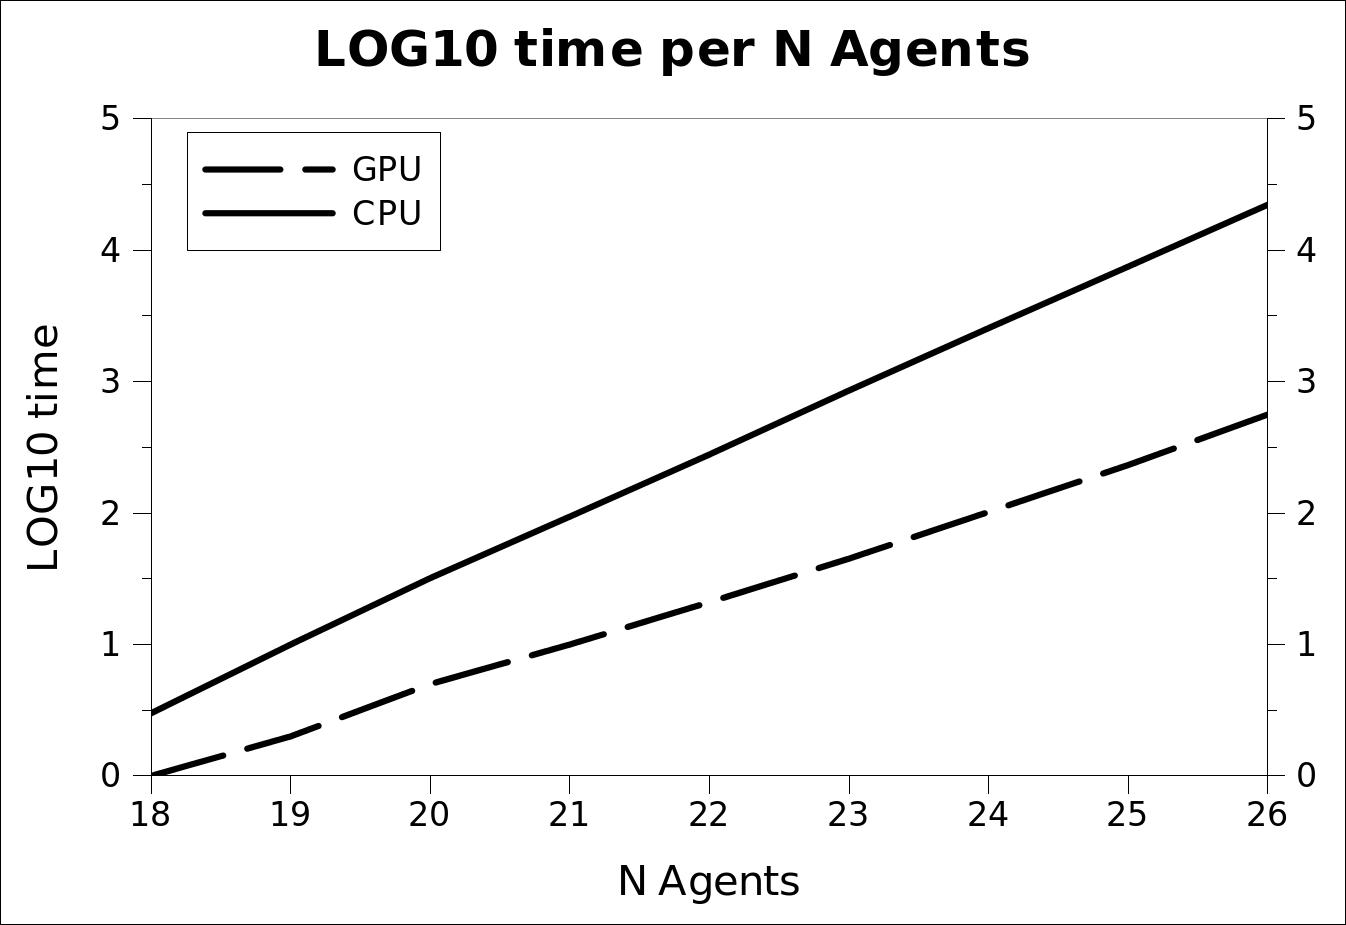
\includegraphics[width=0.7\linewidth]{loggraph.jpg}
\caption{LOG10 runtime per N Agents\label{log}}
\end{figure}
\begin{figure}[htb]
\centering
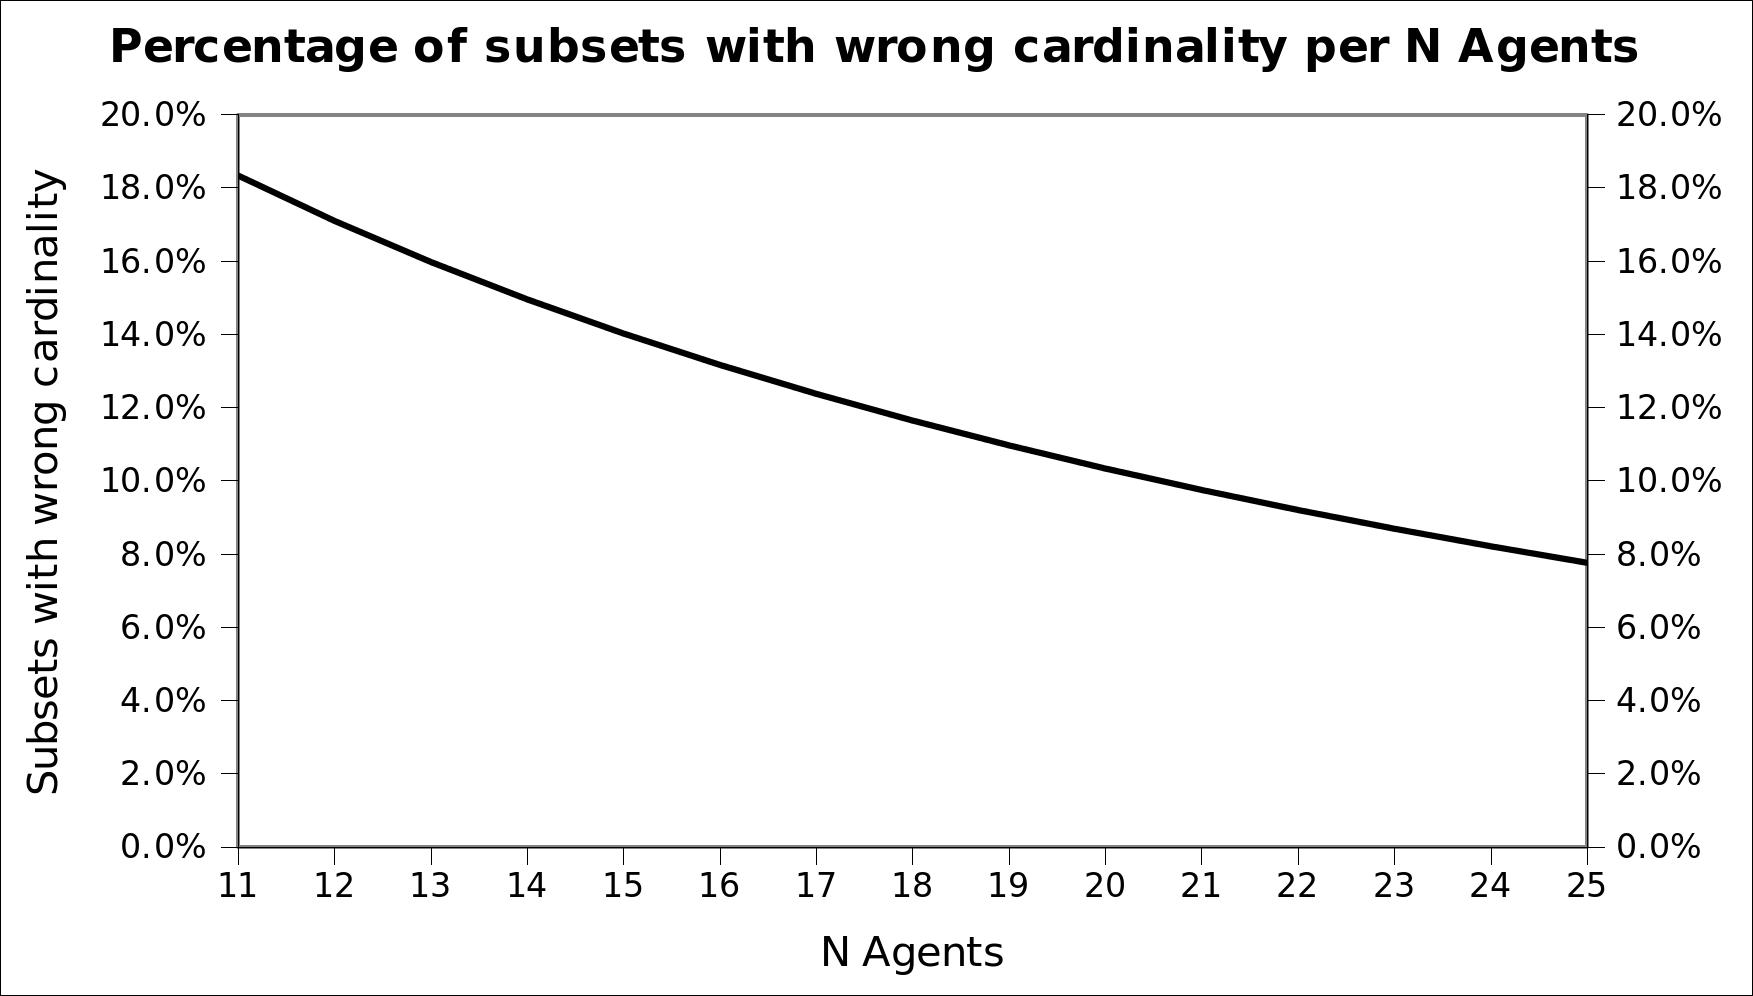
\includegraphics[width=0.7\linewidth]{subset.jpg}
\caption{Percentage of generated subset of wrong cardinality\label{overhead}}
\end{figure}
\subsection{Evaluation}
As it stands now, the algorithm that is running using the CUDA framework have an substantial performance increase as shown in figure~\ref{log}. As seen from the figure, the slope of line CPU and GPU is different, indicating an different growth rate for an increase of n, thus having a different time complexity. Empirical measurement show that for each increase in n, the runtime for the cpu increase by three. While the GPU bound algorithm starts its growth at 2 and the growth increases to 2.42 for 25 agents.

Figure~\ref{overhead} is the evaluation of line~\ref{lst:line:subset} on how many susbsets generated that invalidates the condition $\vert C'_{i} \vert \leq \dfrac{\vert C\vert }{2}$ where $C'_i \subset C$. This is a measure that describe the instruction overhead for that particular part of the algorithm, and as it stands now with the algorithm being limited by memory latency due to random access, this instruction overhead can be considered negligible. This measure however does not take into account any duplicate subsets that are occasionally generated.
\section{Future work}
As there is currently a selected number of algorithms that is regarded faster than the DP algorithm such as the IDP algorithm \citep{rahwan2008improved} that have shown a prommising efficiency. The next step would be to implement it both on the CPU and GPU. However as it is fairly simmilar to the DP algorithm, implementation may be trivial and further goals need to be determined. As the current work only works for a small number of agents, the next step would be to implement an algorithm to solve more realistic combinatoral auctions with an relative large number of agents and low number of coalition structures.

\bibliographystyle{plain}
\bibliography{ref}
\end{document}
